\documentclass[a4paper,twocolumn,twoside,10pt]{article}
\usepackage{graphicx,amsmath,amssymb,amsthm}

\makeatletter \oddsidemargin-.25in \evensidemargin-.25in
\makeatother \topmargin-0.75in \textwidth7in \textheight9.5in

% Place your Latex macros here -----------------------------
% THEOREMS -------------------------------------------------------
\newtheorem{thm}{Theorem}[section]
\newtheorem{cor}{Corollary}[section]
\newtheorem{prob}{Problem}[section]
\newtheorem{lem}{Lemma}[section]
\newtheorem{prop}{Proposition}[section]
\theoremstyle{definition}
\newtheorem{defn}{Definition}[section]
\newtheorem{rem}{Remark}[section]
\newtheorem{ex}{Example}[section]

% MATH -----------------------------------------------------------
\newcommand{\norm}[1]{\left\Vert#1\right\Vert}
\newcommand{\trnorm}[1]{\left\Vert#1\right\Vert_{\mathbf{tr}}}
\newcommand{\abs}[1]{\left\vert#1\right\vert}
\newcommand{\set}[1]{\left\{#1\right\}}
\newcommand{\Real}{\mathbb R}
\newcommand{\eps}{\varepsilon}
\newcommand{\To}{\longrightarrow}
\newcommand{\BX}{\mathbf{B}(X)}
\newcommand{\tr}[1]{\text{tr}\left[#1\right]}
\newcommand{\maxeig}[1]{\mathbf{\lambda_{\max}}\left(#1\right)}
\newcommand{\mineig}[1]{\mathbf{\lambda_{\min}}\left(#1\right)}
\newcommand{\e}[1]{\text{E}\left[#1\right]}
\newcommand{\diag}[1]{\text{diag}\left\{#1\right\}}
\newcommand{\A}{\mathcal{A}}


% Running Head----------------------------------------------------------------
\markboth{$~$ \hfill {\rm Author(s) Name} \hfill $~$} {$~$ \hfill
{\rm Short Title of the Paper} \hfill$~$}

\pagestyle{myheadings} 
%\setcounter{page}{151}


\begin{document}
\def \thepage {}
\date{}

% Title----------------------------------------------------------------
\title{\begin{flushleft}
\noindent {\small {\it Proceedings of ICCSA 2014
\\Normandie University, Le Havre, France - June 23-26, 2014\\[5mm]
 }}
% \noindent {\small {\it Journal of Nonlinear Systems and Applications
% (2009)
% 151--154\\
%  Copyright $\copyright$ 2009 Watam Press \hfill http://www.watam.org/JNSA/\\[5.0mm]}}
\end{flushleft}\Large\bf \uppercase{Robust exponential stability of uncertain switched stochastic systems with
time-delay} }
%\author{\Large\bf Author Index}
\author{Author1, Author2 and Author3
 \thanks{Author1 and Author2 are with  Department of
Applied Mathematics, University of Waterloo, Canada. E-mails:
jnsa@uwaterloo.ca, john@uwaterloo.ca}
\thanks{ Author3 is with  Department of Civil and Environmental Engineering,
University of Waterloo, Canada.  E-mail: david@uwaterloo.ca}
\thanks{Manuscript received April 19, 2009; revised January 11, 2010.}}
 \maketitle

% Abstract----------------------------------------------------------------


{\footnotesize \noindent {\bf Abstract.}  The abstract should be
informative, precise and not exceed
200 words. Please do not include equations, tables and references in the abstract. \\
{\bf Keywords.} At least 5 key words should be provided.}

\vskip.2in

% Contents----------------------------------------------------------------

% ----------------------------------------------------------------
\section{Introduction}
Authors are required to state clearly the contributions of the paper
in the Introduction. There should be some survey of relevant
literature.

Submission of a manuscript by the authors implies
that the paper has not been previously published in any language and
in any form, has not been copyrighted or submitted simultaneously
for publication elsewhere, and that the copyright for the article
will be transferred to the publisher upon acceptance of the article.
The corresponding authors' e-mail addresses must be
included in the manuscript.

Please make sure that all equations and figures do not run off the
margins. Figures and Tables should be placed as part of the text, with descriptive captions and should be numbered consecutively. For LaTeX users, only standards commands are allowed.

The following is taken from various papers, including figures without scientific meaning. The purpose is to show various editing usages. 


Stochastic dynamic modeling plays an
essential role in numerous physics and engineering problems. It can
be applied wherever random properties of a dynamical system have to
be considered. Most of the emphasis is placed on the stability
analysis of the stochastic dynamical systems (see
\cite{Arnold}). Moreover, in many applications,
the physical or chemical processes are governed by more than one
dynamics: the dynamics change among a family of choices with respect
to time $t$ or state $x$. Such processes are often described by
switched systems and have been studied extensively in recent years
(see \cite{Cheng, daaf}). Time-delay and uncertainties are two
main causes for instability of dynamical systems (see
\cite{Boyd}). Numerous studies have been carried out on
stability analysis and stabilization of time-delay systems and
uncertain systems (see
\cite{Cao,Chen}), some of which have
been done in the scope of stochastic systems or switched systems. To
the best knowledge of the authors, few work has been done for
switched stochastic systems with both uncertainties and time-delay.
Some results are given by the figure \ref{onesurface}.

\begin{figure}[htp]
\centering
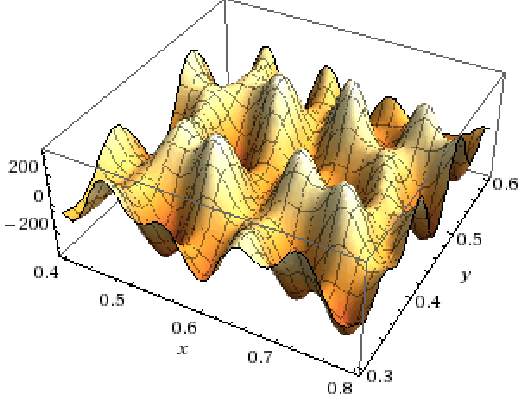
\includegraphics[width=0.4\textwidth]{surface.pdf}
\caption{A beautiful surface}
\label{onesurface}
\end{figure}


\section{Problem statement and preliminaries}\label{sec2}
\subsection{Formulation}
Consider the following stochastic uncertain switched system
\begin{align}
dx(t)&=[(A_i+\Delta A_i)x(t)+(\tilde{A_i}+\Delta\tilde{
A_i})x(t-h)]dt\nonumber\\
&\quad+[(B_i+\Delta B_i)x(t)+(\tilde{B_i}+\Delta\tilde{
B_i})x(t-h)]dw(t),\notag\\
&\qquad\qquad\text{for}\quad
t\geq0,\,\alpha(t)=i,\label{sw_sy}
\\[1\jot]
x(t)&=\phi(t),\,t\in [-h,0],\nonumber
\end{align}
where $x\in\Real^n$ is the state and $h$ is the constant time-delay.\\

\begin{figure*}[htp]
\centering
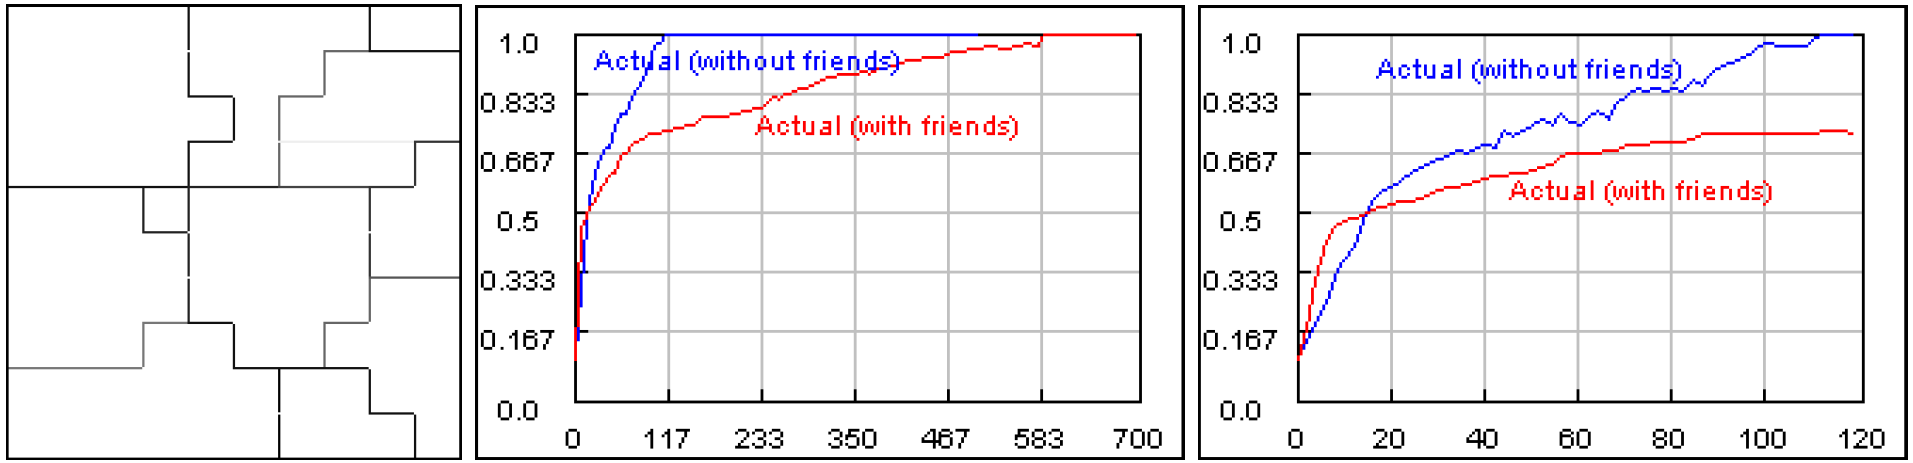
\includegraphics[width=0.8\textwidth]{experiment1.png}
\caption{In this first experiment, typical outcome for a modified homogeneous Axelrod model is presented. (Left) An intermediate configuration in the case of partner selection. (Middle) Actual affinities with and without friends (partner selection). (Right) Zoom to the first part of the previous graph (first 120 cycles).}
\label{experiment1} 
\end{figure*}

In the following, we describe some experiments.\\

\textbf{Experiment 1}. Modified Axelrod model (homogeneous) results with an initially diverse population
(fig. \ref{experiment1}). Partner selection does not change the final outcome which is full monoculture in the
population, but it substantially retards the cultural contagion process. On the other hand, partner
selection induces extremely fast local polarization as is depicted in fig. \ref{experiment1}(left) where an intermediate
configuration is shown, that is not possible without partner selection in this model. Fig. \ref{experiment1}(right)
shows the large speed of local convergence in the beginning of the experiment that slows down in
what follows compared to the convergence speed without partner selection.\\

\textbf{Experiment 2}. Modified Axelrod model (homogeneous) with two initial populations where a
cultural clash is expected. Again, partner selection does not change the final outcome which is full
monoculture in the population, but it substantially retards the cultural contagion process. This is due
to the border agents between the two populations that create individualistic partnerships and thus
hinder the fast spreading of cultural information.\\

\subsection{Stability}

Two types of stability are considered in this paper, one is almost
sure exponential stability and the other is exponential stability in
$p$th moment (see \cite{Cheng} for definitions). The main problem
now can be formulated as follows:
\begin{prob}
For all admissible uncertainties, under what conditions will the
uncertain switched system $(\ref{sw_sy})$ be almost surely
exponentially stable? Under what conditions will it be exponentially
stable in mean square?
\end{prob}

\section{Main results}\label{sec3}
In this section, the stability analysis of system (\ref{sw_sy}) is
studied.

The following
matrix inequalities are satisfied:
\begin{align}
\Psi_i=\begin{bmatrix}
\Psi_{11}&\Psi_{12}&\Psi_{13}\\
\star&\Psi_{22}&\Psi_{23}\\
\star&\star&\Psi_{33}
\end{bmatrix}&<0,\label{ineq11}\\
Q_i&\leq\rho_iI\label{ineq12},
\end{align}


\section{Application}\label{sec4}

\begin{table}
\caption{Stability bounds of time-delay and average dwell time}\label{table2}
\begin{center}
{\tt
\begin{tabular}{|c||c|c|c|c|}
\hline $T_0\,\,(\times 10^3)$& $0$ & $0.0856$ & $0.2303$ & $0.7960$\\
\hline $h_0$& $0$ & $0.5$ & $1.0$ & $1.5$\\
\hline $T_0\,\,(\times 10^3)$ &$1.7645$& $3.0717$ & $5.1803$ & $9.2734$\\
\hline $h_0$& $2.0$&$2.5$ & $3.0$ & $3.5$\\
\hline $T_0\,\,(\times 10^3)$ &$23.4052$& $238.2837$ & $$ & $$\\
\hline $h_0$& $4.0$&$4.4$ & $$ & $$\\
\hline
\end{tabular}
}
\end{center}
\end{table}

For different average
dwell time lower bounds $T_0$, the delay upper bounds $h_0$
guaranteeing the exponential stability of the system are listed in
Table \ref{table2}.


\section*{Acknowledgements}
The research for this work was supported, in part, by the Natural
Sciences and Engineering Research Council of Canada.

\footnotesize

% Bibliography----------------------------------------------------------------
\begin{thebibliography}{1}
\bibitem{Arnold}L.~Arnold, \emph{Stochastic Differential Equations: Theory
and Applications}, John Wiley and Sons, 1974.
\bibitem{Boyd}S.~Boyd, L.~E.~Ghaoui, E.~Feron, and V.~Balakrishnan,
\emph{Linear Matrix Inequalities in System and Control Theory},
SIAM, Philadephia, 1994.
\bibitem{Cao}Y.~Y.~Cao, Y.~X.~Sun, and C.~Cheng, ``Delay-dependent robust stabilization of uncertain systems with multiple state
delays,'' \emph{IEEE Transactions on Automat. Control}, vol. 43, pp.
1608-1612, 1998.
\bibitem{Chen}W.-H.~Chen, Z.~H.~Guan, X.~Lu, ``Delay-dependent exponential stability of uncertain stochastic
systems with multiple delays: an LMI approach,'' \emph{Systems
Control Lett.}, vol. 54, pp. 547-555, 2005.
\bibitem{Cheng}
D.~Cheng, ``Stabilization of planar switched systems'',
\emph{Systems Control Lett.} vol. 51, pp. 79-88, 2004.
\bibitem{daaf}
J.~Daafouz, P.~Riedinger, C.~Iung, ``Stability analysis and control
synthesis for switched systems: a switched Lyapunov function
approach'', \emph{IEEE Trans. Automat. Control}, vol. 47, pp.
1883-1887, 2002.
\end{thebibliography}


\end{document}
% ----------------------------------------------------------------
